% ---------------------------------------------------------------------------
% Author guideline and sample document for EG publication using LaTeX2e input
% D.Fellner, v1.15, Dec 14, 2018
% \httpAddr{//docs.miktex.org/manual/} 
\documentclass{egpubl}
\usepackage{gch2020}

% --- for  Annual CONFERENCE
% \ConferenceSubmission   % uncomment for Conference submission
% \ConferencePaper        % uncomment for (final) Conference Paper
% \STAR                   % uncomment for STAR contribution
% \Tutorial               % uncomment for Tutorial contribution
% \ShortPresentation      % uncomment for (final) Short Conference Presentation
% \Areas                  % uncomment for Areas contribution
% \MedicalPrize           % uncomment for Medical Prize contribution
% \Education              % uncomment for Education contribution
% \Poster                 % uncomment for Poster contribution
% \DC                     % uncomment for Doctoral Consortium
%
% --- for  CGF Journal
% \JournalSubmission    % uncomment for submission to Computer Graphics Forum
% \JournalPaper         % uncomment for final version of Journal Paper
%
% --- for  CGF Journal: special issue
% \SpecialIssueSubmission    % uncomment for submission to , special issue
% \SpecialIssuePaper         % uncomment for final version of Computer Graphics Forum, special issue
%                          % EuroVis, SGP, Rendering, PG
% --- for  EG Workshop Proceedings
 \WsSubmission      % uncomment for submission to EG Workshop
% \WsPaper           % uncomment for final version of EG Workshop contribution
% \WsSubmissionJoint % for joint events, for example ICAT-EGVE
% \WsPaperJoint      % for joint events, for example ICAT-EGVE
% \Expressive        % for SBIM, CAe, NPAR
% \DigitalHeritagePaper
% \PaperL2P          % for events EG only asks for License to Publish

% --- for EuroVis 
% for full papers use \SpecialIssuePaper
% \STAREurovis   % for EuroVis additional material 
% \EuroVisPoster % for EuroVis additional material 
% \EuroVisShort  % for EuroVis additional material

% !! *please* don't change anything above
% !! unless you REALLY know what you are doing
% ------------------------------------------------------------------------
\usepackage[T1]{fontenc}
\usepackage{dfadobe}  
\usepackage{multirow}

\usepackage{cite}  % comment out for biblatex with backend=biber
% ---------------------------
%\biberVersion
\BibtexOrBiblatex
%\usepackage[backend=biber,bibstyle=EG,citestyle=alphabetic,backref=true]{biblatex} 
%\addbibresource{egbibsample.bib}
% ---------------------------  
\electronicVersion
\PrintedOrElectronic
% for including postscript figures
% mind: package option 'draft' will replace PS figure by a filename within a frame
\ifpdf \usepackage[pdftex]{graphicx} \pdfcompresslevel=9
\else \usepackage[dvips]{graphicx} \fi

\usepackage{egweblnk} 
\hypersetup{breaklinks=true}
% end of prologue
\usepackage{amsmath}
\usepackage{pseudocode}
\usepackage[ruled]{algorithm2e}
 \usepackage[usenames,dvipsnames]{xcolor}
 \usepackage[normalem]{ulem}  % for strike-through (\sout)


\input twmacros
% ---------------------------------------------------------------------
% EG author guidelines plus sample file for EG publication using LaTeX2e input
% D.Fellner, v2.03, Dec 14, 2018
\title[Heritage in lockdown: digital provision of memory institutions during the Covid-19 crisis]%
      {Heritage in lockdown: digital provision of memory institutions in the United Kingdom and United States during the Covid-19 crisis}

% for anonymous conference submission please enter your SUBMISSION ID
% instead of the author's name (and leave the affiliation blank) !!
% for final version: please provide your *own* ORCID in the brackets following \orcid; see https://orcid.org/ for more details.
% \author[D. Fellner \& S. Behnke]
% {\parbox{\textwidth}{\centering D.\,W. Fellner\thanks{Chairman Eurographics Publications Board}$^{1,2}$\orcid{0000-0001-7756-0901}
%         and S. Behnke$^{2}$\orcid{0000-0001-5923-423X} 
% %        S. Spencer$^2$\thanks{Chairman Siggraph Publications Board}
%         }
%         \\
% % For Computer Graphics Forum: Please use the abbreviation of your first name.
% {\parbox{\textwidth}{\centering $^1$TU Darmstadt \& Fraunhofer IGD, Germany\\
%          $^2$Graz University of Technology, Institute of Computer Graphics and Knowledge Visualization, Austria
% %        $^2$ Another Department to illustrate the use in papers from authors
% %             with different affiliations
%        }
% }
% }
% ------------------------------------------------------------------------

% if the Editors-in-Chief have given you the data, you may uncomment
% the following five lines and insert it here
%
% \volume{36}   % the volume in which the issue will be published;
% \issue{1}     % the issue number of the publication
% \pStartPage{1}      % set starting page


%-------------------------------------------------------------------------
\begin{document}

\teaser{
 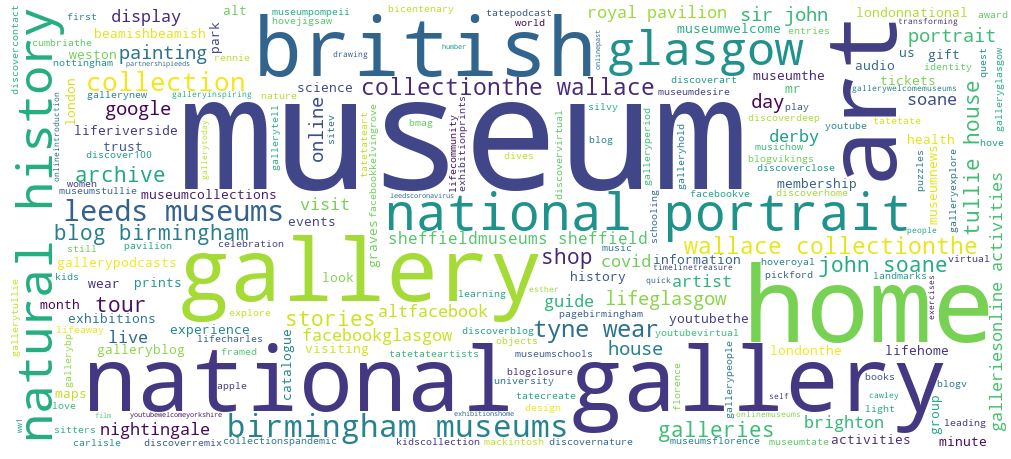
\includegraphics[width=0.6\linewidth]{images/cloud.png}
 \centering
  \caption{Word cloud of common keywords for digital offerings of memory institutions during COVID-19 lockdown}
\label{fig:teaser}
}

\maketitle
%-------------------------------------------------------------------------
\begin{abstract}
   The ABSTRACT is to be in fully-justified italicized text, 
   between two horizontal lines,
   in one-column format, 
   below the author and affiliation information. 
   Use the word ``Abstract'' as the title, in 9-point Times, boldface type, 
   left-aligned to the text, initially capitalized. 
   The abstract is to be in 9-point, single-spaced type.
   The abstract may be up to 3 inches (7.62 cm) long. \\
   Leave one blank line after the abstract, 
   then add the subject categories according to the ACM Classification Index 
%-------------------------------------------------------------------------
%  ACM CCS 1998
%  (see https://www.acm.org/publications/computing-classification-system/1998)
% \begin{classification} % according to https://www.acm.org/publications/computing-classification-system/1998
% \CCScat{Computer Graphics}{I.3.3}{Picture/Image Generation}{Line and curve generation}
% \end{classification}
%-------------------------------------------------------------------------
%  ACM CCS 2012
   (see https://www.acm.org/publications/class-2012)
%The tool at \url{http://dl.acm.org/ccs.cfm} can be used to generate
% CCS codes.
%Example:
\begin{CCSXML}
<ccs2012>
<concept>
<concept_id>10010147.10010371.10010352.10010381</concept_id>
<concept_desc>Computing methodologies~Collision detection</concept_desc>
<concept_significance>300</concept_significance>
</concept>
<concept>
<concept_id>10010583.10010588.10010559</concept_id>
<concept_desc>Hardware~Sensors and actuators</concept_desc>
<concept_significance>300</concept_significance>
</concept>
<concept>
<concept_id>10010583.10010584.10010587</concept_id>
<concept_desc>Hardware~PCB design and layout</concept_desc>
<concept_significance>100</concept_significance>
</concept>
</ccs2012>
\end{CCSXML}

\ccsdesc[300]{Computing methodologies~Collision detection}
\ccsdesc[300]{Hardware~Sensors and actuators}
\ccsdesc[100]{Hardware~PCB design and layout}


\printccsdesc   
\end{abstract}  
%-------------------------------------------------------------------------
\section{Introduction}
Museums and heritage institutions are a key element for society, especially during crises, such as the outbreak of the COVID-19 pandemic. Such institutions not only are vital for the communities they serve as research and knowledge centres, evidencing the past and present of tangible and intangible heritage; but, most importantly, form part of the communities' identity as they are an essential part of people's identity as well as a vital element for the communities by empowering people, especially in times of uncertainty such as the health crisis we experience today and its socioeconomic ramifications \cite{ICOM:2020}.

As the impact of COVID-19 on everyday lives dawned on people early in 2020, digital media consumption behaviour changed dramatically as millions of people tried to cope with the realities imposed by the lockdown. The UK reported a 29\% increase on the time spent online, and a 20\% increase of people using social media \cite{ofcom:2020}. 

Within the COVID-19 crisis, the majority of work sectors have been affected by restrictions of physical access and limited provision of services during lockdowns. As expected, the galleries, libraries, archives, and museums (GLAM) sector could not stay unaffected by the crisis. Apart from the immediate effect on museums' workforce and finances, organisations have had to close, postpone or cancel projects, exhibitions and art programmes that they offer to their audiences. Despite these difficulties, the sector has demonstrated remarkable resilience by adapting their digital provision to allow online access to arts and culture in order to reduce isolation, improve mental health and support the educational and creative needs of diverse audiences.

The research that this paper presents was conducted during the lockdown period in the UK, from early spring to summer 2020, when museums started to gradually re-open their physical premises to visitors. The aim of the research was to understand how the cultural heritage institutions have adapted during lockdowns by developing their digital cababilities; how these developments ``translate" into actual digital offerings that enable to access cultural heritage resources; what are the audiences that institutions target and how their distinctive needs have been met during the COVID-19 pandemic. In order to acquire a more complete image of the sector's adaptation to the COVID-19 crisis, the research incorporated a comparative assessment of international responses during the lockdown by collecting and analysing data from institutions in the United States of America (USA). Deploying such approach can be justified as i) both countries have a variety of museums and heritage organisations with relatively good levels of expertise and capacity in terms of digital technologies; ii) the lockdown in the UK and USA followed a similar timeline (whether this was country/state-wide or happened on a phased basis) with ``stay-at-home'' suggestions from mid-March onwards; and iii) both countries encounter similar socioeconomic challenges where heritage could make a difference or play a role.

The research was conducted by an interdisciplinary team developing a methodology to record data through an extensive survey of digital offerings on the web and then analysing them quantitatively, while providing useful insights through qualitative analysis as well. The development of the research and its results are reported in this paper. The paper’s main contributions include: i) a unique record and useful insight into memory institutions’ digital offerings during a three-month strict lockdown period for the UK and USA; and ii) an in-depth analysis of the institutions' response to a crisis, which has the potential to inform future IT developments to keep heritage content relevant to societal needs. For instance, the analysis of data allows us to identify trends and novel ways of enabling access to heritage resources which might prove transformational in the following years.

The paper is organised as follows: Section X describes the context and related work in this area; while section X presents the methodology which was deployed for conducting the research and capturing data. Section X analyses the findings of the research. Finally, Section X presents conclusions and further work.  

%-------------------------------------------------------------------------
\section{Context and related work}
As the COVID-19 pandemic started to engulf the planet in the first months of 2020, a response from governments, institutions, industries and consequently the GLAM sector was generated in order to adapt to the new reality imposed by local or nation-wide lockdowns. The following subsections describe contextual information with regards to the immediate response of major heritage organisations and their guidance towards museums and cultural heritage institutions during closures. Related work illuminating the impact of COVID-19 on the sector is also mentioned here.

\subsection{Context}
Museum closures due to the COVID-19 pandemic started around mid-March 2020 with The Wellcome Collection in the UK and the Metropolitan Museum of Art (MET) being amongst the first ones that announced that they were shutting down \textbf{(McGivern 2020, the art newspaper & Kendall Adams, museum association 2020)}. Around the same time, some of the major heritage  associations started investigating plans in order to cope with the uncertainty of closures while continuing to support communities during these difficult times. For instance, the American Alliance of Museums proposed three scenarios with different levels of impact (low, medium and high) to assist organisations to develop their own response to the crisis. These scenarios would work as the framework to manage risks in the best possible way, while supporting communities and their well-being, protecting the museum workforce and planning for the financial impact of the pandemic \textbf{(Merritt AAm-us 2020)}.

Since then, guidance from organisations such as the Museums Association in the UK and the International Council of Museums (ICOM) would highlight similar challenges and steer the sector's adaptation by prioritising \textbf{(museums and covid-19 8 steps, icom & ma practical ways museums can contribute & covid-19:urgent demands to rpotect museum workers 17.3.202 ma)}:

\begin{itemize}
\item the financial viability of heritage institutions through calls for support
\item the security of collections and the safety of staff
\item practical support of health systems by donating equipment and volunteering 
\item alternative or innovative approaches to conduct activities that cannot take place in the physical space, including new ways of working, revisiting of traditional tools and new communication channels with audiences
\item responses to societal needs and current developments, including supporting vulnerable groups such as the homeless, people suffering from dementia, children who cannot access easily education, refugees, minorities and women experiencing domestic violence
\item partnerships between institutions in the heritage sector and beyond as well as collaborations with local communities (often with emphasis on health, well-being, justice and sustainability)
\item learning from solidarity, empathy and resilience as emerged during similar situations in the past (e.g. physical catastrophes) or societal topics (e.g. human rights, conflicts and other)
\item reconsideration of accessibility standards and procedures
\item collection and documentation of the current crisis and its impact
\item reflection on the COVID-19 experience and revisiting priorities, strengths, weaknesses and practices possibly transforming the future of organisations
\item advocacy initiatives by the sector's bodies in order to secure funding and protection for organisations.
\end{itemize}

Apart, though, from setting the above priorities, heritage associations launched further guidance to reach and support audiences during the health crisis. Some of the suggested means of remote engagement are \textbf{(3 references ICOM, AAM, NEMO)}:

\begin{itemize}
\item online collections by offering access to digital copies or artwork (often through Open Access), exhibitions and more

\item virtual tours by deploying social media platforms, such as Facebook, Instagram Live, Pinterest curated content, Twitter threads, YouTube Live

\items podcasts to facilitate audio tours in exhibitions, discussions about the collections and analysis of interesting topics

\item social media campaigns, challenges and quizzes often with a humorous spirit by using hashtags to encourage people to share their stories (e.g. #MuseumFromHome, #BetweenArtandQuarantine)

\item live streams of educational activities, creative sessions, story times and more through social media and other live event platforms

\item VR/AR experiences and 3D object exploration

\end{itemize}







all the above....demarialise the focus of insitutions 




The new reality  in 
Presentation of situation for museums, what are the main challenges (funding, civic museums-those under a Trust, resilience, recovery of communities, reopening)
What are the main suggestions from cultural organisations and bodies to help museums cope with Covid. Mention here what are the aspects they prioritise (requirements).
Lara might want to add on wellbeing here.
Might add about social inclusion here (see ICOM museum day celebration)


\subsection{Related Work}
The surveys that organisations such as ICOM, UNESCO, NEMO, Art Fund, Heritage Fund have published. What do they demonstrate (key findings with respect to digital offerings).
We might want to add somewhere here that there is research about the digital offerings from major organisations analysing the digital provision during lockdown, but we have to emphasize that we look at it from the “opposite” side, by actually analysing the offerings further and seeing their relation to audiences. Also we might want to emphasize that this research not only provides an in-depth examination of the digital provision, but might also highlight key trends about the digital future of museums and new ways of funcion.

%-------------------------------------------------------------------------

\section{Methodology}
-> How we created the list of museums, and strategies for recording.
Research questions:
What  was being offered? By whom?
Does the data demonstrate if offerings match needs that have emerged?
The research questions which were investigated are as follows:
1) Which web-based digital provision was available to audiences during the UK lockdown period by UK and US museums? 
2) Which traditional and non-traditional audiences that this digital provision was targeting?
3) Which types of content museums engaged, ranging from text-based to more complex spatial-visual types of content, including Virtual Reality and panoramic images?
4) How museums seek financial support from audiences?
5) How museums kept content relevant to peoples’ challenges, including isolation, mental wellbeing and inclusivity?

Match questions to the questions in introduction when we finalise them.
Here we need to analyse:
Classification of offerings under type and subtype (a table could also show what these are)
Audiences (specific reference to Covid audiences) and what they are
Sample selection 
What type of analysis do we use and validity / triangulation (data triangulation: museums in two countries, national, small, civic, special theme museums \& “investigator” /analyst  triangulation: more than one researchers to collect and classify and analyse data)

%-------------------------------------------------------------------------

%\section{Data Capture}
Capturing the data for the research involved surveying memory institutions’ websites as described above. In total, we surveyed 83 memory institutions both in the UK and the US (48 institutions in the  UK and 35 institutions in the US). The selection included major institutions from both countries (e.g. based on visitor numbers in wikipedia) plus a selection of smaller civic, historic and/or city museums. For this additional selection, we made use of the National Museums Director Council in the UK \cite{nationalmuseums:2020}; and made a selection of smaller museums in different states of the US. For some memory institutions, which are aggregated under an umbrella trust, we surveyed the umbrella organisation as in most cases the COVID response is the same in smaller organisations as in the biggest one of the same consortium/trust (with one or two different resources sometimes).

When surveying, researchers followed a strategy to identify what digital offering was deemed to be a COVID-19 response, as opposed to traditional website content. This was very difficult in some cases, as many institutions re-purposed or sign-posted existing content as being COVID-19 relevant. This was not surprising given how relevant memory institutions are for the educational, well-being, and self-improving needs of communities. Thus, most organisations restructured their content to address the pandemic by creating COVID-19 “highlights” or “sliders” on their front pages. These new pages allowed users to reach a variety of relevant content instead of reaching the content through the traditional website menu structure. The variety of COVID-19 resources in each institution was vast, and researchers followed these highlighted routes to identify which digital offerings were relevant for the survey.

Furthermore, it was not straightforward to identify the impact that the digital offering had on users. This is because it is difficult to measure access to web pages without having access to museums’ web teams. Exceptions are the number of views on websites such as YouTube, followers in social media, or number of downloads in sites such as SketchFab. However, even these were difficult to directly relate as being COVID-19 specific as most content was available before the lockdown. Instead we undertook a different approach by recording all URL to digital offerings. With these URLs, we were able to query the keywords made available on the web page titles and analyse the popularity of keywords in search queries in Google Search across various regions and languages. 

In order to offer a meaningful classification of the results, we adopted different classification and sub-classification including: the types of digital offering, the type of audiences, the type of content, the type of memory institutions and types of donations which institutions were requesting during this period. These are described below.

\subsection{Digital offerings classification}
An important task of data capture was to design an appropriate classification for digital offerings. This classification had to enable researchers to record as accurately as possible the purpose of the content which was being offered to visitors during the COVID-19 lockdown period. As mentioned previously, a large majority of the content was not specific to COVID-19 related topics. Hence, the classification was generic to deal with a variety of offerings by memory institutions. Table~\ref{tab:digoffer} shows this classification, which categorizes offerings into seven categories: collection, virtual visit, learning, home activities, events, funding and communication. Inevitably, there is overlap between different categories as access to the collection could enable learning or be a home activity. However, we categorise digital offerings according to how the content was being presented using a variety of keywords to highlight its purpose. 

Also, Table~\ref{tab:digoffer} shows a subtype classification we designed to further classify each type of digital offering. This was particularly important for understanding the types of access to the collection being offered, the types of events memory institutions organised and the types of communication strategies they used during this period. Thus, subtypes of the ``Collection'' type digital offering could include: free database exploration, guided exploration, collection related resources, 3D collection, image database/resources as well as collecting content. The latter was particularly of interest as some memory institutions set to actively collect digital content or objects from the public during the lockdown period.

\begin{table}
\begin{tabular}
{ | l | l | }
    \hline
    Digital Offering Type  & Subtype  \\
    \hline
  \multirow{6}{*}{Collection} & Free database exploration  \\
&  Guided exploration  \\
&  Collection related resources \\
&  3D collection \\
&  Images database/resources \\
&  Collecting content \\
    \hline
 \multirow{2}{*}{Virtual visit} & Gallery tour  \\
&  Audio tour  \\
    \hline
 Learning & Educational material  \\
    \hline
 \multirow{2}{*}{Home activities} & Creative activities \\
&  Wellbeing activities  \\
    \hline
 \multirow{4}{*}{Events} & Festival\\
&  Live event \\
&  Other \\
&  Competition \\
    \hline
 Funding & comercial venture \\
    \hline
 \multirow{12}{*}{Communication} & COVID-19 communication \\
& Podcast \\
& Blog/articles' section \\
& Social media  \\
& Videos \\
& Student/artist resources \\
& Racism related \\
& Practical info \\
& Digital publications \\
& Practical info \\
& Music lists \\
& Other \\
    \hline
\end{tabular}
\caption{\label{tab:digoffer}Digital offering types and subtypes used in the survey}
\end{table}

\subsection{COVID-19 audiences}
As a means to understand which traditional and non-traditional audiences the digital offering which memory institutions provided was being targeted, we created a segmentation of COVID-19 relevant audiences. Although, it will have been possible to adapt existing segmentations used by institutions already \cite{Drot19}; instead we adopted Jones \cite{Audiences2020} proposed COVID-19 audience segmentation. This segmentation takes into account how digital offerings of memory institutions fulfil emotional needs of people affected by the pandemic. As such the classification distinguishes between people who have specific educational (e.g., teachers, learners, parents doing home schooling), well-being issues (e.g. lonely or grieving  people, bored), beyond traditional museum audiences (e.g. local community, internal and museum audiences). The types of audiences include: Bored people, Desperate parents \& children, Teachers at sea, Higher education/Professional teaching online, Eager learners, Stressed out/scared people, Grieving people, People who can’t stop working on their job sites, Museum constituencies (specific interest/core audiences for content), Museum members/donors, Local community, Lonely people, Working from Home / Newly unemployed, People wanting to help others, Internal audiences.

\subsection{Types of content}
To further understand what the digital offering consists of, the survey recorded a description of the offering and a type of content. Although most webpages consists of text and image elements, we also recorded whether the offering included more complex data types, such as video (including live video stream), audio, 360º virtual tour and interactive panorama/VR/AR type experiences, 3D objects or interactive games and activities. The latter visual types of content were of particular interest, as they allow for audiences to engage more actively with the digital offering. They can either allow audiences to explore the collection, and/or to the exhibition physical space; for example, images of the collection, interactive panoramic tours,  behind the scenes audiovisual material, and virtual galleries/visit. Besides being a popular type of content, visual content has some advantages for audiences, such as being more inclusive to multiple understandings and interpretations, as well as overcoming communication barriers, such as language and attention barriers. However, it can also be less accessible for those with disabilities if the content has not been designed appropriately.

\subsection{Sample selection}
The survey included a variety of memory institutions’ types illustrated in Figure~\ref{fig:MType}. Some institutions were recorded under two or more categories, either because they present a variety of collections or to address the fact that we selected umbrella organisations who oversee different types of smaller institutions. The data recorded for each museum also included the city and country where the museum was located, as well as a Wikidata code so that more information could be retrieved during the analysis phase.

\subsection{Funding and donations}
Given the importance of memory institutions’ finances during the COVID-19 crisis, the survey recorded specific data regarding whether some institutions highlighted potential ways audiences could contribute to support financially the museum. Hence, the survey also recorded calls for donations in relationship to the COVID-19 needs of institutions. Although many institutions normally request for donations, we recorded whether there was a specific COVID-19 message when requesting donations. For this, we recorded different types of funding, including i) call for donations emphasising (or not)  COVID-19, ii) call to support through other means, such as shop purchases, memberships or gifts; and iii) or when there was no specific call for donations.

Beside the types previously described, data was also recorded - when available, regarding the author and date of creation of the digital offering, its URL and any additional comment which was worth recording. Data was recorded from April the 23rd 2020, only one month after the UK went into lockdown, until the 31st of July 2020, a few weeks after museums and galleries were allowed to reopen to the public. The following subsection will present and analyse the resulting data. 

%-------------------------------------------------------------------------

\section{Findings}
The analysis of the data collected allowed us to explore in detail the digital offerings of memory institutions during the COVID-19 lockdown period in order to answer the research questions. To recap, these questions related to: 1) the types of digital offerings, and the nature of the content, which was available to audiences; 2) the types of audiences these offerings targeted; 4) the financial support sought by museums from audiences; and 3) exploring how the digital offerings matched needs that emerged during the COVID-19 pandemic in particular with regards to peoples’ challenges, including isolation, mental well-being and inclusivity. 

A total of 922 digital offerings were recorded as offering relevant content for the COVID-19 lockdown amongst all memory institutions. This includes a total of 515 digital offerings in the UK, and 407 digital offerings in the US; with an average of 11 digital offerings per memory institutions. We reiterate that not all of this content was newly created, but could have been highlighted as relevant to the perceived needs of audiences. 


The following subsections will analyse different aspects of the data including the memory institutions, the types of offerings, the audiences and financial issues.

\subsection{Memory institutions surveyed}
As Figure~\ref{fig:MType} illustrates the survey included a mixture of institutions ranging from History/Historic house or place (18\%), Art (14\%), Art and History (12\%), Polythematic (10\%), Museum Trust (8\%), Special Theme (8\%), Science (8\%), Maritime/Military (8\%), Natural History (7\%), and Library/Archive (5\%). Within these variety of institutions, there are representatives of different types of collections, galleries, exhibitions and historic environments; all of which can be experienced through a variety of digital offerings. 


\begin{figure}[h]
  \centering
  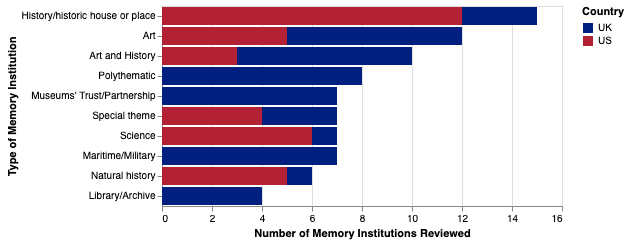
\includegraphics[width=\linewidth]{images/museumtype.png}
  % replacing the above command with the one below will explicitly set
  % the bounding box of the PS figure to the rectangle (xl,yl),(xh,yh).
  % It will also prevent LaTeX from reading the PS file to determine
  % the bounding box (i.e., it will speed up the compilation process)
  % 
\includegraphics[width=.95\linewidth, bb=39 696 126 756]{sampleFig}
  %
  % \parbox[t]{.9\columnwidth}{\relax
  %          For all figures please keep in mind that you \textbf{must not}
  %          use images with transparent background! 
  %          }
  %
  \caption{\label{fig:MType}
           Types of memory institutions surveyed}
\end{figure}

Moreover, Figure~\ref{fig:typeofferings} presents the number of digital offerings recorded for each type of memory institution. In average, History/Historic houses provided 10 offerings, Art institutions provided 12 offerings, Art and history institutions provided 13 offerings, Polythematic institutions provided 14 offerings, Museum Trusts provided 9 offerings, Special Theme institutions provided 10 offerings, Science institutions provided 11 offerings, Maritime/Military institutions provided 11 offerings, Natural History institutions provided 12 and Library/Archive institutions provided 12 offerings. 

\begin{figure}[h]
  \centering
  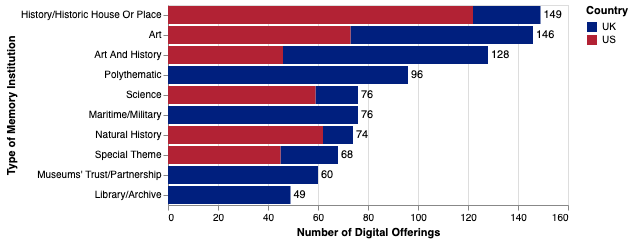
\includegraphics[width=\linewidth]{images/typesoffering.png}
  \caption{\label{fig:typeofferings}
           Number of digital offerings provided by different types of institutions}
\end{figure}



% 922 total

\subsection{Digital offerings}
With regards to types of digital offerings, Figure~\ref{fig:DigOffType} shows the number of digital offerings classified according to their type. Furthermore, Figures~\ref{fig:MTypeOfferings} cross-relates the number of offerings types with the different types of memory institutions which provided them. As both of these figure shows, digital offerings of \emph{Communication} (43\%) and \emph{Collection} (28\%) type were the most popular. 

The figure illustrates that digital offerings both for providing access to memory institutions' collection and communicating with audiences were the most popular both in the UK and the US. This demonstrates the value which memory institutions place on enabling access to collection content in terms of fulfilling their remit throughout the lockdown period. In addition, memory institutions actively seek to keep in contact with audiences during the lockdown period. This also confirms that memory institutions responded well to advice to keep communication with audiences via alternative channels of communication through digital tools and platforms. 


Also of interest, is the fact there  were so few virtual visits being offered, despite the fact audiences could not physically visit memory institutions. Probably, the biggest barrier for this was the lack of content of such experiences. Some examples of virtual visits which were provided include last minute videos of the curator of Michelangelo's exhibition at the Getty Museum in empty rooms before the museum's closure \cite{getty2020}.

The less explored type of digital offering relates to \emph{Funding}, with only 4\% of the digital offerings related to this aspect. This is somehow surprising given how the lack of funding might affect memory institutions post-COVID-19. Although, there is also an element of lack of digital offerings or business models which can allow memory institutions to generate additional funding. Interesting examples were found regarding digital offerings which are commercial ventures, includes recipe boxes to buy with all the ingredients and instructions to prepare food at home offered by Birmingham Museum \& Art Gallery; or genealogy search services offered by the Statue of Liberty-Ellis Island Foundation which provided research to trace family history/arrival to America by the institution research staff. Also, there were some museums which generated income by organising ticketed live events, such as the online science camp for pupils organised by California Science Centre.

% 60 digital offerings amongst 7 institutions, with an average of 8 offerings), given their overall representation in the sample  

% 49 /

% 60 /


\begin{figure}[h]
  \centering
  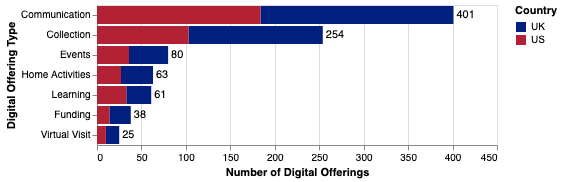
\includegraphics[width=\linewidth]{images/digitalTypes.png}
  \caption{\label{fig:DigOffType}
           Types of digital offerings during the COVID-19 period}
\end{figure}




\begin{figure}[h]

  \centering
  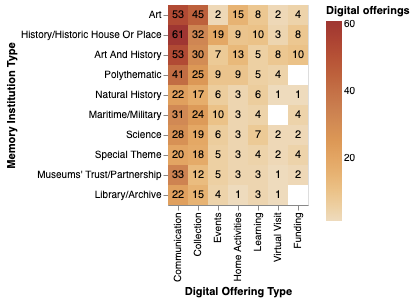
\includegraphics[width=\linewidth]{images/museumoffering.png}
  \caption{\label{fig:MTypeOfferings}
           Types of digital offerings provided by types of institutions }
\end{figure}



% 679 eager learners
% 417 teachers
% 19 grieving - 2%
% 12 PWTHO - 2%
% 922 total

\subsection{Audiences}

Figures~\ref{fig:MTypeAudiences} presents the number of offerings targeted to specific audiences by each type of memory institution both in the UK and the US. The data illustrates the strong emphasis on memory institutions addressing educational needs of audiences during the pandemic, with a strong focus on audiences who seek opportunities to gain new knowledge, such as teachers and higher education academics, as well as learners in both countries. For instance, the data highlights how \emph{Eager learners} were the most dominant type of audiences with 74\% of digital offerings. Audiences created by COVID-19, such as those grieving (2\%) or wanting to help others, e.g. carers, (2\%) where those less directly targeted by offerings.

\begin{figure}[h]
  \centering
  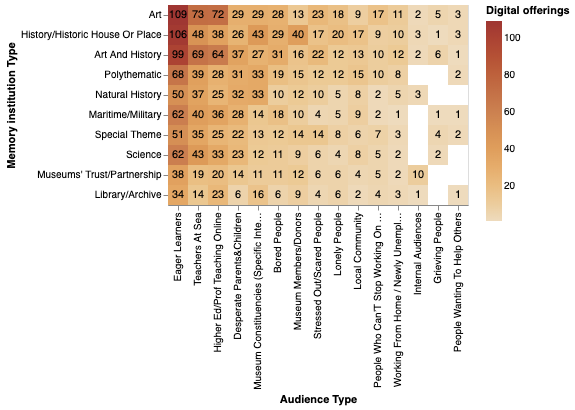
\includegraphics[width=\linewidth]{images/audiencesboth.png}
  \caption{\label{fig:MTypeAudiences}
           Types of audiences targeted by types of institutions }
\end{figure}



This data suggests that most memory institutions focused primordially on traditional audiences;  rather than those newly created during the COVID-19 pandemic, including lonely or grieving people. It also confirms that institutions might have re-purposed material, already available, which support core aims of these institutions as knowledge providers for audiences. As a result, it is noted a lack of digital offerings focusing on tackling specific well-being and emotional needs of these type of audiences. Some interesting example  of this  type of offerings includes physical activity packs which were offered by the Exeter Royal Albert Memorial Museum \& Art Gallery to shielded, vulnerable and isolated people in the city to help ease lockdown boredom \cite{ex2020}; as well as a ``Cultural First Aid kit'', developed by Manchester Museum, focusing on well-being for people in hospitals and care centres \cite{man2020}. 

% Table~ref

% \begin{figure}[h]
%   \centering
%   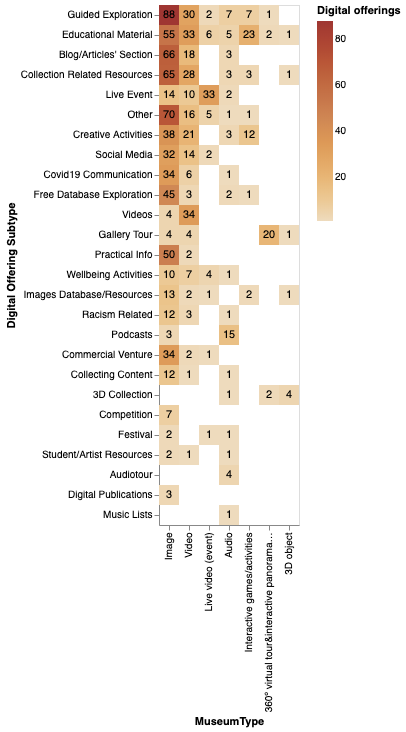
\includegraphics[width=\linewidth]{images/typescontent.png}
%   % replacing the above command with the one below will explicitly set
%   % the bounding box of the PS figure to the rectangle (xl,yl),(xh,yh).
%   % It will also prevent LaTeX from reading the PS file to determine
%   % the bounding box (i.e., it will speed up the compilation process)
%   % 
\includegraphics[width=.95\linewidth, bb=39 696 126 756]{sampleFig}
%   % %
%   % \parbox[t]{.9\columnwidth}{\relax
%   %          For all figures please keep in mind that you \textbf{must not}
%   %          use images with transparent background! 
%   %          }
%   %
%   \caption{\label{fig:MTypeAudiences}
%            Types of Content made available by institutions both in the UK and the US.}
% \end{figure}

Moreover, Figure~\ref{fig:Subtypeaudiences} shows digital offerings for three distinct groups of audiences, which have been classified according to their primordial needs: 

\begin{itemize}
	\item emotional and entertainment  \emph{(left)}
	\item educational \emph{centre}
	\item stakeholder involvement \emph{right}
\end{itemize}

 subtypes of digital offerings for the \emph{Collection} type of digital offering. The total of offerings for guided exploration represented the largest amount. Of interest are those collection and resources which were addressing  societal concerns during the COVID-19 lockdown period, including the Black Live Matters activism movement in the UK and the US. \KR{Do we have an interesting example of resources offered?}

%For instance, the San Francisco Museum of Modern Art(SFMOMA) statement about artists who have recalled their work from the museum's website as a response to the Black Lives Matter protests.
% \begin{figure}[h]
%   \centering
%   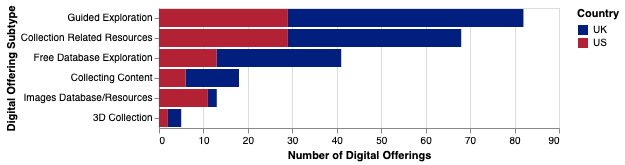
\includegraphics[width=\linewidth]{images/collection.png}
%   \caption{\label{fig:Collection}
%            Subtypes of digital offerings of Collection type }
% \end{figure}


\begin{figure*}[h]
  \centering
  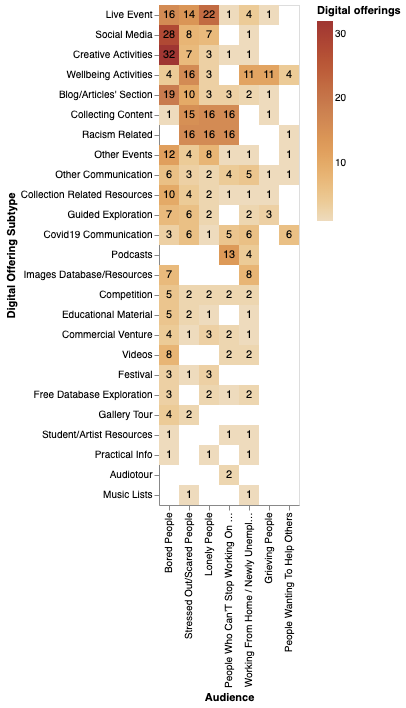
\includegraphics[width=.34\linewidth]{images/emotionalneeds.png}
  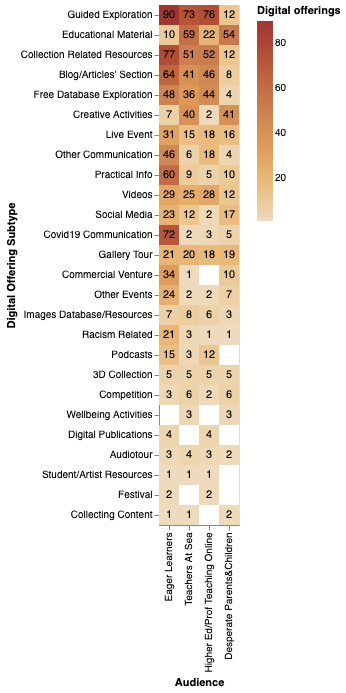
\includegraphics[width=.29\linewidth]{images/educationneeds.png}
  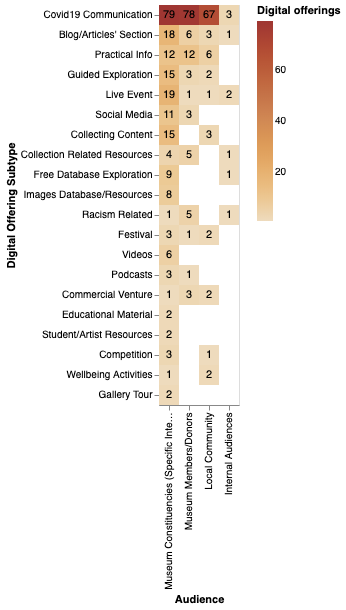
\includegraphics[width=.32\linewidth]{images/internalneeds.png}
  \caption{\label{fig:Subtypeaudiences} Audiences-based digital offerings classified according to the primordial audiences needs: emotional and entertainment  \emph{(left)}, educational \emph{centre}, stakeholder involvement \emph{right}}

\end{figure*}

\color{red}To answer:
Which museums target groups that need support through wellbeing activities
How many museums collected content 
\color{black}

However, there is less evidence on how these digital provision might have reached or engaged with some of the groups identified under risk, such as women at risk of domestic violence, children with difficult access to education, migrants, refugees, unemployed, health workers and minorities experiencing increased discrimination and xenophobia. 
% \begin{figure}[h]
%   \centering
%   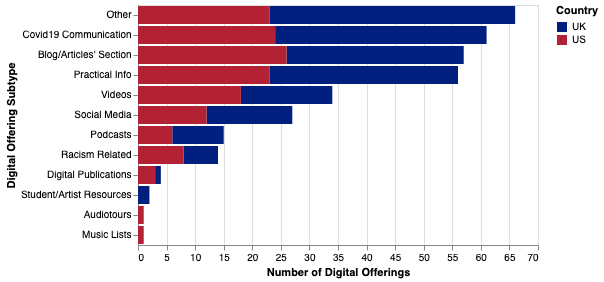
\includegraphics[width=\linewidth]{images/communication.png}
%   \caption{\label{fig:DigOffType2}
%            Subtypes of digital offerings of Commuincation type}
% \end{figure}

\color{red}To answer: Data  categorised  as  type of museum - do focus on wellbeing happening by certain types of museums?\color{black}

\begin{figure}[h]
  \centering
  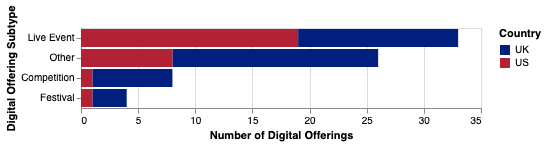
\includegraphics[width=\linewidth]{images/event.png}
  \caption{\label{fig:DigOffType3} 
           Subtypes of digital offerings of Event type}
\end{figure}

\subsection{Audiences targetted by digital provision}
\color{red}To answer: Which audience is mostly targeted for the overall provision?\color{black}

% \begin{figure}[h]
%   \centering
%   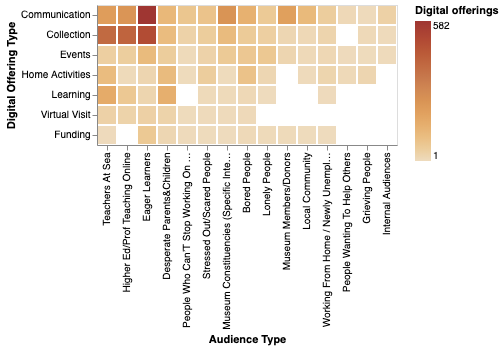
\includegraphics[width=\linewidth]{images/typeaudience.png}
%   \caption{\label{fig:DigOffType4}
%            Types of digital offerings targetted to different audiences
%            }
% \end{figure}

% \begin{figure}[h]
%   \centering
%   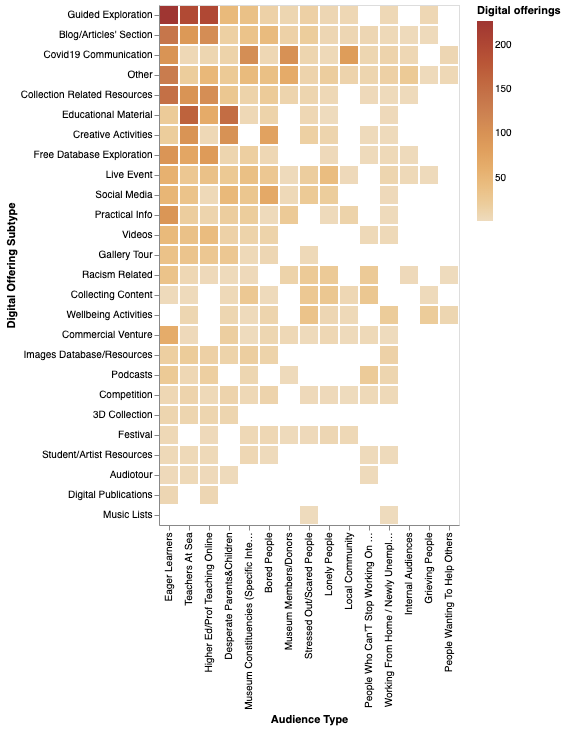
\includegraphics[width=\linewidth]{images/subtypeaudience.png}
%   \caption{\label{fig:DigOffType5}
%                       Types of digital offerings targetted to different audiences}

% \end{figure}

\noindent \textbf{Content for audiences}
\color{red}To answer: Which is the strongest/more popular format ?\color{black}


% \begin{figure}[h]
%   \centering
%   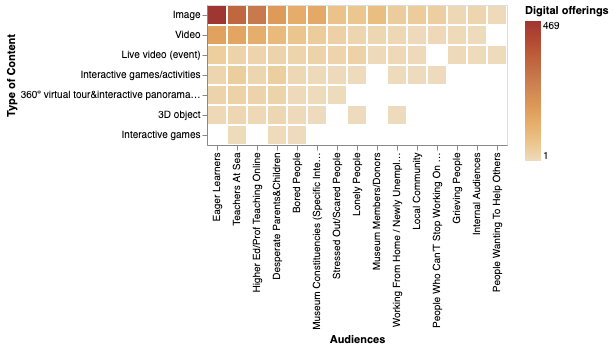
\includegraphics[width=\linewidth]{images/contentaudience.png}
%   \caption{\label{fig:DigOffType6}
%                       Types of content provided to different audiences}

% \end{figure}

\subsection{Funding and donations}
\color{red}To answer: What do data show about donation campaigns?\color{black}



\subsection{Interesting offerings }
Demonstrate some of the novelties that have emerged (look at section 3 of my document and add to categories below)
Also: 
Curators’ view and tours in exhibitions to give a “personal touch” (plus last minute “emergency” tours before closure)
Covid related content collection (to document the health crisis)
Monetizing digital offerings (income generating)
Connection to other sites and cultural institutions (solidarity)
Well being, mental health focus, mention the very limited examples that offer physical offerings for those  that do not have access to the digital provision.
Surveys about the future of digital offerings and reopening
Decolonisation, Black lives matter
Which digital offering request for payment? (I think this cannot be added here, but rather in the section of “special offerings”)

\section{Discussion and conclusions}
Identified gaps:
More training/skills are required to fulfill the novel digital requirements (digital literacy within the house). Freelancers have been amongst the first groups who stopped working for museums and there is no financial capacity to pay for freelancers' work (even though these were often assisting with digital work before the covid crisis). In order to adapt to the situation in house staff have had to take on new responsibilities. Also, digital inequality between big and smaller/rural museums is evident in reports and funding for digital activities is minimum (see section 7 of my document).
Marketing opportunities  - how can museums produce revenue from digital offerings. How people have monetised digital offerings? (look at Money list article)
Lack of agreed methods and metrics to measure digital engagement (mention relevant research and efforts -e.g. The audience agency- but there is no consensus).
Future development:
How can this content have a legacy beyond the lockdown and how the priorities of the sector might change (focus on digital instead of physical, communication between staff, more flexible working, diversity and inclusion because of flexible working, use of external spaces for exhibitions etc?)
How local strategies can be developed to build resilience especially for older people (at home or in care homes), shielding people, people with mental health issues, grieving communities etc (mention access to physical activities too). 
How digital can help not only audiences, but the way the museums work and function under the new normal? (Contactless interactives; Own mobile device tour apps; Visitor flow management; Virtual tours and the virtual museum.)
Issues that have have not been adequately addressed during the crisis:
Services/offerings for disabled audiences (could also make reference to our work with blind audiences an 3d prints that could be offered as a “print on demand” service in a similar way that museums offer prints of works of art). Generally lack of special provision (physical objects, sign language, look at Vocal Eyes newsletters)
Diversity and decolonisation through/for the digital provision by addressing the sparsity of current efforts (maybe mention the SFMOMA examples here as well).

-> any discussion regarding what future work is of interest, and conclusions
->  how things might evolve
Future work will include to develop a better  understanding on how audiences engaged with this type of content  , and the impact that it is having on audiences. 





% %%%
% %%% Figure 1
% %%%
% \begin{figure}[htb]
%   \centering
%   % the following command controls the width of the embedded PS file
%   % (relative to the width of the current column)
%   
\includegraphics[width=.8\linewidth]{sampleFig}
%   % replacing the above command with the one below will explicitly set
%   % the bounding box of the PS figure to the rectangle (xl,yl),(xh,yh).
%   % It will also prevent LaTeX from reading the PS file to determine
%   % the bounding box (i.e., it will speed up the compilation process)
%   % 
\includegraphics[width=.95\linewidth, bb=39 696 126 756]{sampleFig}
%   %
%   \parbox[t]{.9\columnwidth}{\relax
%            For all figures please keep in mind that you \textbf{must not}
%            use images with transparent background! 
%            }
%   %
%   \caption{\label{fig:firstExample}
%            Here is a sample figure.}
% \end{figure}


%-------------------------------------------------------------------------
% bibtex
\bibliographystyle{eg-alpha-doi}  
\bibliography{egbibsample}        

% biblatex with biber
% \printbibliography                

%-------------------------------------------------------------------------


\end{document}

